
% Default to the notebook output style

    


% Inherit from the specified cell style.




    
\documentclass[11pt]{article}

    
    
    \usepackage[T1]{fontenc}
    % Nicer default font (+ math font) than Computer Modern for most use cases
    \usepackage{mathpazo}
	\usepackage{float}
    % Basic figure setup, for now with no caption control since it's done
    % automatically by Pandoc (which extracts ![](path) syntax from Markdown).
    \usepackage{graphicx}
    % We will generate all images so they have a width \maxwidth. This means
    % that they will get their normal width if they fit onto the page, but
    % are scaled down if they would overflow the margins.
    \makeatletter
    \def\maxwidth{\ifdim\Gin@nat@width>\linewidth\linewidth
    \else\Gin@nat@width\fi}
    \makeatother
    \let\Oldincludegraphics\includegraphics
    % Set max figure width to be 80% of text width, for now hardcoded.
    \renewcommand{\includegraphics}[1]{\Oldincludegraphics[width=.8\maxwidth]{#1}}
    % Ensure that by default, figures have no caption (until we provide a
    % proper Figure object with a Caption API and a way to capture that
    % in the conversion process - todo).
    \usepackage{caption}
    \DeclareCaptionLabelFormat{nolabel}{}
    \captionsetup{labelformat=nolabel}

    \usepackage{adjustbox} % Used to constrain images to a maximum size 
    \usepackage{xcolor} % Allow colors to be defined
    \usepackage{enumerate} % Needed for markdown enumerations to work
    \usepackage{geometry} % Used to adjust the document margins
    \usepackage{amsmath} % Equations
    \usepackage{amssymb} % Equations
    \usepackage{textcomp} % defines textquotesingle
    % Hack from http://tex.stackexchange.com/a/47451/13684:
    \AtBeginDocument{%
        \def\PYZsq{\textquotesingle}% Upright quotes in Pygmentized code
    }
    \usepackage{upquote} % Upright quotes for verbatim code
    \usepackage{eurosym} % defines \euro
    \usepackage[mathletters]{ucs} % Extended unicode (utf-8) support
    \usepackage[utf8x]{inputenc} % Allow utf-8 characters in the tex document
    \usepackage{fancyvrb} % verbatim replacement that allows latex
    \usepackage{grffile} % extends the file name processing of package graphics 
                         % to support a larger range 
    % The hyperref package gives us a pdf with properly built
    % internal navigation ('pdf bookmarks' for the table of contents,
    % internal cross-reference links, web links for URLs, etc.)
    \usepackage{hyperref}
    \usepackage{longtable} % longtable support required by pandoc >1.10
    \usepackage{booktabs}  % table support for pandoc > 1.12.2
    \usepackage[inline]{enumitem} % IRkernel/repr support (it uses the enumerate* environment)
    \usepackage[normalem]{ulem} % ulem is needed to support strikethroughs (\sout)
                                % normalem makes italics be italics, not underlines
    \usepackage{mathrsfs}
    

    
    
    % Colors for the hyperref package
    \definecolor{urlcolor}{rgb}{0,.145,.698}
    \definecolor{linkcolor}{rgb}{.71,0.21,0.01}
    \definecolor{citecolor}{rgb}{.12,.54,.11}

    % ANSI colors
    \definecolor{ansi-black}{HTML}{3E424D}
    \definecolor{ansi-black-intense}{HTML}{282C36}
    \definecolor{ansi-red}{HTML}{E75C58}
    \definecolor{ansi-red-intense}{HTML}{B22B31}
    \definecolor{ansi-green}{HTML}{00A250}
    \definecolor{ansi-green-intense}{HTML}{007427}
    \definecolor{ansi-yellow}{HTML}{DDB62B}
    \definecolor{ansi-yellow-intense}{HTML}{B27D12}
    \definecolor{ansi-blue}{HTML}{208FFB}
    \definecolor{ansi-blue-intense}{HTML}{0065CA}
    \definecolor{ansi-magenta}{HTML}{D160C4}
    \definecolor{ansi-magenta-intense}{HTML}{A03196}
    \definecolor{ansi-cyan}{HTML}{60C6C8}
    \definecolor{ansi-cyan-intense}{HTML}{258F8F}
    \definecolor{ansi-white}{HTML}{C5C1B4}
    \definecolor{ansi-white-intense}{HTML}{A1A6B2}
    \definecolor{ansi-default-inverse-fg}{HTML}{FFFFFF}
    \definecolor{ansi-default-inverse-bg}{HTML}{000000}

    % commands and environments needed by pandoc snippets
    % extracted from the output of `pandoc -s`
    \providecommand{\tightlist}{%
      \setlength{\itemsep}{0pt}\setlength{\parskip}{0pt}}
    \DefineVerbatimEnvironment{Highlighting}{Verbatim}{commandchars=\\\{\}}
    % Add ',fontsize=\small' for more characters per line
    \newenvironment{Shaded}{}{}
    \newcommand{\KeywordTok}[1]{\textcolor[rgb]{0.00,0.44,0.13}{\textbf{{#1}}}}
    \newcommand{\DataTypeTok}[1]{\textcolor[rgb]{0.56,0.13,0.00}{{#1}}}
    \newcommand{\DecValTok}[1]{\textcolor[rgb]{0.25,0.63,0.44}{{#1}}}
    \newcommand{\BaseNTok}[1]{\textcolor[rgb]{0.25,0.63,0.44}{{#1}}}
    \newcommand{\FloatTok}[1]{\textcolor[rgb]{0.25,0.63,0.44}{{#1}}}
    \newcommand{\CharTok}[1]{\textcolor[rgb]{0.25,0.44,0.63}{{#1}}}
    \newcommand{\StringTok}[1]{\textcolor[rgb]{0.25,0.44,0.63}{{#1}}}
    \newcommand{\CommentTok}[1]{\textcolor[rgb]{0.38,0.63,0.69}{\textit{{#1}}}}
    \newcommand{\OtherTok}[1]{\textcolor[rgb]{0.00,0.44,0.13}{{#1}}}
    \newcommand{\AlertTok}[1]{\textcolor[rgb]{1.00,0.00,0.00}{\textbf{{#1}}}}
    \newcommand{\FunctionTok}[1]{\textcolor[rgb]{0.02,0.16,0.49}{{#1}}}
    \newcommand{\RegionMarkerTok}[1]{{#1}}
    \newcommand{\ErrorTok}[1]{\textcolor[rgb]{1.00,0.00,0.00}{\textbf{{#1}}}}
    \newcommand{\NormalTok}[1]{{#1}}
    
    % Additional commands for more recent versions of Pandoc
    \newcommand{\ConstantTok}[1]{\textcolor[rgb]{0.53,0.00,0.00}{{#1}}}
    \newcommand{\SpecialCharTok}[1]{\textcolor[rgb]{0.25,0.44,0.63}{{#1}}}
    \newcommand{\VerbatimStringTok}[1]{\textcolor[rgb]{0.25,0.44,0.63}{{#1}}}
    \newcommand{\SpecialStringTok}[1]{\textcolor[rgb]{0.73,0.40,0.53}{{#1}}}
    \newcommand{\ImportTok}[1]{{#1}}
    \newcommand{\DocumentationTok}[1]{\textcolor[rgb]{0.73,0.13,0.13}{\textit{{#1}}}}
    \newcommand{\AnnotationTok}[1]{\textcolor[rgb]{0.38,0.63,0.69}{\textbf{\textit{{#1}}}}}
    \newcommand{\CommentVarTok}[1]{\textcolor[rgb]{0.38,0.63,0.69}{\textbf{\textit{{#1}}}}}
    \newcommand{\VariableTok}[1]{\textcolor[rgb]{0.10,0.09,0.49}{{#1}}}
    \newcommand{\ControlFlowTok}[1]{\textcolor[rgb]{0.00,0.44,0.13}{\textbf{{#1}}}}
    \newcommand{\OperatorTok}[1]{\textcolor[rgb]{0.40,0.40,0.40}{{#1}}}
    \newcommand{\BuiltInTok}[1]{{#1}}
    \newcommand{\ExtensionTok}[1]{{#1}}
    \newcommand{\PreprocessorTok}[1]{\textcolor[rgb]{0.74,0.48,0.00}{{#1}}}
    \newcommand{\AttributeTok}[1]{\textcolor[rgb]{0.49,0.56,0.16}{{#1}}}
    \newcommand{\InformationTok}[1]{\textcolor[rgb]{0.38,0.63,0.69}{\textbf{\textit{{#1}}}}}
    \newcommand{\WarningTok}[1]{\textcolor[rgb]{0.38,0.63,0.69}{\textbf{\textit{{#1}}}}}
    
    
    % Define a nice break command that doesn't care if a line doesn't already
    % exist.
    \def\br{\hspace*{\fill} \\* }
    % Math Jax compatibility definitions
    \def\gt{>}
    \def\lt{<}
    \let\Oldtex\TeX
    \let\Oldlatex\LaTeX
    \renewcommand{\TeX}{\textrm{\Oldtex}}
    \renewcommand{\LaTeX}{\textrm{\Oldlatex}}
    % Document parameters
    % Document title
    \title{Assignment 6}
    
    
    \author{Jiarong Ye}
    
    
    

    % Pygments definitions
    
\makeatletter
\def\PY@reset{\let\PY@it=\relax \let\PY@bf=\relax%
    \let\PY@ul=\relax \let\PY@tc=\relax%
    \let\PY@bc=\relax \let\PY@ff=\relax}
\def\PY@tok#1{\csname PY@tok@#1\endcsname}
\def\PY@toks#1+{\ifx\relax#1\empty\else%
    \PY@tok{#1}\expandafter\PY@toks\fi}
\def\PY@do#1{\PY@bc{\PY@tc{\PY@ul{%
    \PY@it{\PY@bf{\PY@ff{#1}}}}}}}
\def\PY#1#2{\PY@reset\PY@toks#1+\relax+\PY@do{#2}}

\expandafter\def\csname PY@tok@w\endcsname{\def\PY@tc##1{\textcolor[rgb]{0.73,0.73,0.73}{##1}}}
\expandafter\def\csname PY@tok@c\endcsname{\let\PY@it=\textit\def\PY@tc##1{\textcolor[rgb]{0.25,0.50,0.50}{##1}}}
\expandafter\def\csname PY@tok@cp\endcsname{\def\PY@tc##1{\textcolor[rgb]{0.74,0.48,0.00}{##1}}}
\expandafter\def\csname PY@tok@k\endcsname{\let\PY@bf=\textbf\def\PY@tc##1{\textcolor[rgb]{0.00,0.50,0.00}{##1}}}
\expandafter\def\csname PY@tok@kp\endcsname{\def\PY@tc##1{\textcolor[rgb]{0.00,0.50,0.00}{##1}}}
\expandafter\def\csname PY@tok@kt\endcsname{\def\PY@tc##1{\textcolor[rgb]{0.69,0.00,0.25}{##1}}}
\expandafter\def\csname PY@tok@o\endcsname{\def\PY@tc##1{\textcolor[rgb]{0.40,0.40,0.40}{##1}}}
\expandafter\def\csname PY@tok@ow\endcsname{\let\PY@bf=\textbf\def\PY@tc##1{\textcolor[rgb]{0.67,0.13,1.00}{##1}}}
\expandafter\def\csname PY@tok@nb\endcsname{\def\PY@tc##1{\textcolor[rgb]{0.00,0.50,0.00}{##1}}}
\expandafter\def\csname PY@tok@nf\endcsname{\def\PY@tc##1{\textcolor[rgb]{0.00,0.00,1.00}{##1}}}
\expandafter\def\csname PY@tok@nc\endcsname{\let\PY@bf=\textbf\def\PY@tc##1{\textcolor[rgb]{0.00,0.00,1.00}{##1}}}
\expandafter\def\csname PY@tok@nn\endcsname{\let\PY@bf=\textbf\def\PY@tc##1{\textcolor[rgb]{0.00,0.00,1.00}{##1}}}
\expandafter\def\csname PY@tok@ne\endcsname{\let\PY@bf=\textbf\def\PY@tc##1{\textcolor[rgb]{0.82,0.25,0.23}{##1}}}
\expandafter\def\csname PY@tok@nv\endcsname{\def\PY@tc##1{\textcolor[rgb]{0.10,0.09,0.49}{##1}}}
\expandafter\def\csname PY@tok@no\endcsname{\def\PY@tc##1{\textcolor[rgb]{0.53,0.00,0.00}{##1}}}
\expandafter\def\csname PY@tok@nl\endcsname{\def\PY@tc##1{\textcolor[rgb]{0.63,0.63,0.00}{##1}}}
\expandafter\def\csname PY@tok@ni\endcsname{\let\PY@bf=\textbf\def\PY@tc##1{\textcolor[rgb]{0.60,0.60,0.60}{##1}}}
\expandafter\def\csname PY@tok@na\endcsname{\def\PY@tc##1{\textcolor[rgb]{0.49,0.56,0.16}{##1}}}
\expandafter\def\csname PY@tok@nt\endcsname{\let\PY@bf=\textbf\def\PY@tc##1{\textcolor[rgb]{0.00,0.50,0.00}{##1}}}
\expandafter\def\csname PY@tok@nd\endcsname{\def\PY@tc##1{\textcolor[rgb]{0.67,0.13,1.00}{##1}}}
\expandafter\def\csname PY@tok@s\endcsname{\def\PY@tc##1{\textcolor[rgb]{0.73,0.13,0.13}{##1}}}
\expandafter\def\csname PY@tok@sd\endcsname{\let\PY@it=\textit\def\PY@tc##1{\textcolor[rgb]{0.73,0.13,0.13}{##1}}}
\expandafter\def\csname PY@tok@si\endcsname{\let\PY@bf=\textbf\def\PY@tc##1{\textcolor[rgb]{0.73,0.40,0.53}{##1}}}
\expandafter\def\csname PY@tok@se\endcsname{\let\PY@bf=\textbf\def\PY@tc##1{\textcolor[rgb]{0.73,0.40,0.13}{##1}}}
\expandafter\def\csname PY@tok@sr\endcsname{\def\PY@tc##1{\textcolor[rgb]{0.73,0.40,0.53}{##1}}}
\expandafter\def\csname PY@tok@ss\endcsname{\def\PY@tc##1{\textcolor[rgb]{0.10,0.09,0.49}{##1}}}
\expandafter\def\csname PY@tok@sx\endcsname{\def\PY@tc##1{\textcolor[rgb]{0.00,0.50,0.00}{##1}}}
\expandafter\def\csname PY@tok@m\endcsname{\def\PY@tc##1{\textcolor[rgb]{0.40,0.40,0.40}{##1}}}
\expandafter\def\csname PY@tok@gh\endcsname{\let\PY@bf=\textbf\def\PY@tc##1{\textcolor[rgb]{0.00,0.00,0.50}{##1}}}
\expandafter\def\csname PY@tok@gu\endcsname{\let\PY@bf=\textbf\def\PY@tc##1{\textcolor[rgb]{0.50,0.00,0.50}{##1}}}
\expandafter\def\csname PY@tok@gd\endcsname{\def\PY@tc##1{\textcolor[rgb]{0.63,0.00,0.00}{##1}}}
\expandafter\def\csname PY@tok@gi\endcsname{\def\PY@tc##1{\textcolor[rgb]{0.00,0.63,0.00}{##1}}}
\expandafter\def\csname PY@tok@gr\endcsname{\def\PY@tc##1{\textcolor[rgb]{1.00,0.00,0.00}{##1}}}
\expandafter\def\csname PY@tok@ge\endcsname{\let\PY@it=\textit}
\expandafter\def\csname PY@tok@gs\endcsname{\let\PY@bf=\textbf}
\expandafter\def\csname PY@tok@gp\endcsname{\let\PY@bf=\textbf\def\PY@tc##1{\textcolor[rgb]{0.00,0.00,0.50}{##1}}}
\expandafter\def\csname PY@tok@go\endcsname{\def\PY@tc##1{\textcolor[rgb]{0.53,0.53,0.53}{##1}}}
\expandafter\def\csname PY@tok@gt\endcsname{\def\PY@tc##1{\textcolor[rgb]{0.00,0.27,0.87}{##1}}}
\expandafter\def\csname PY@tok@err\endcsname{\def\PY@bc##1{\setlength{\fboxsep}{0pt}\fcolorbox[rgb]{1.00,0.00,0.00}{1,1,1}{\strut ##1}}}
\expandafter\def\csname PY@tok@kc\endcsname{\let\PY@bf=\textbf\def\PY@tc##1{\textcolor[rgb]{0.00,0.50,0.00}{##1}}}
\expandafter\def\csname PY@tok@kd\endcsname{\let\PY@bf=\textbf\def\PY@tc##1{\textcolor[rgb]{0.00,0.50,0.00}{##1}}}
\expandafter\def\csname PY@tok@kn\endcsname{\let\PY@bf=\textbf\def\PY@tc##1{\textcolor[rgb]{0.00,0.50,0.00}{##1}}}
\expandafter\def\csname PY@tok@kr\endcsname{\let\PY@bf=\textbf\def\PY@tc##1{\textcolor[rgb]{0.00,0.50,0.00}{##1}}}
\expandafter\def\csname PY@tok@bp\endcsname{\def\PY@tc##1{\textcolor[rgb]{0.00,0.50,0.00}{##1}}}
\expandafter\def\csname PY@tok@fm\endcsname{\def\PY@tc##1{\textcolor[rgb]{0.00,0.00,1.00}{##1}}}
\expandafter\def\csname PY@tok@vc\endcsname{\def\PY@tc##1{\textcolor[rgb]{0.10,0.09,0.49}{##1}}}
\expandafter\def\csname PY@tok@vg\endcsname{\def\PY@tc##1{\textcolor[rgb]{0.10,0.09,0.49}{##1}}}
\expandafter\def\csname PY@tok@vi\endcsname{\def\PY@tc##1{\textcolor[rgb]{0.10,0.09,0.49}{##1}}}
\expandafter\def\csname PY@tok@vm\endcsname{\def\PY@tc##1{\textcolor[rgb]{0.10,0.09,0.49}{##1}}}
\expandafter\def\csname PY@tok@sa\endcsname{\def\PY@tc##1{\textcolor[rgb]{0.73,0.13,0.13}{##1}}}
\expandafter\def\csname PY@tok@sb\endcsname{\def\PY@tc##1{\textcolor[rgb]{0.73,0.13,0.13}{##1}}}
\expandafter\def\csname PY@tok@sc\endcsname{\def\PY@tc##1{\textcolor[rgb]{0.73,0.13,0.13}{##1}}}
\expandafter\def\csname PY@tok@dl\endcsname{\def\PY@tc##1{\textcolor[rgb]{0.73,0.13,0.13}{##1}}}
\expandafter\def\csname PY@tok@s2\endcsname{\def\PY@tc##1{\textcolor[rgb]{0.73,0.13,0.13}{##1}}}
\expandafter\def\csname PY@tok@sh\endcsname{\def\PY@tc##1{\textcolor[rgb]{0.73,0.13,0.13}{##1}}}
\expandafter\def\csname PY@tok@s1\endcsname{\def\PY@tc##1{\textcolor[rgb]{0.73,0.13,0.13}{##1}}}
\expandafter\def\csname PY@tok@mb\endcsname{\def\PY@tc##1{\textcolor[rgb]{0.40,0.40,0.40}{##1}}}
\expandafter\def\csname PY@tok@mf\endcsname{\def\PY@tc##1{\textcolor[rgb]{0.40,0.40,0.40}{##1}}}
\expandafter\def\csname PY@tok@mh\endcsname{\def\PY@tc##1{\textcolor[rgb]{0.40,0.40,0.40}{##1}}}
\expandafter\def\csname PY@tok@mi\endcsname{\def\PY@tc##1{\textcolor[rgb]{0.40,0.40,0.40}{##1}}}
\expandafter\def\csname PY@tok@il\endcsname{\def\PY@tc##1{\textcolor[rgb]{0.40,0.40,0.40}{##1}}}
\expandafter\def\csname PY@tok@mo\endcsname{\def\PY@tc##1{\textcolor[rgb]{0.40,0.40,0.40}{##1}}}
\expandafter\def\csname PY@tok@ch\endcsname{\let\PY@it=\textit\def\PY@tc##1{\textcolor[rgb]{0.25,0.50,0.50}{##1}}}
\expandafter\def\csname PY@tok@cm\endcsname{\let\PY@it=\textit\def\PY@tc##1{\textcolor[rgb]{0.25,0.50,0.50}{##1}}}
\expandafter\def\csname PY@tok@cpf\endcsname{\let\PY@it=\textit\def\PY@tc##1{\textcolor[rgb]{0.25,0.50,0.50}{##1}}}
\expandafter\def\csname PY@tok@c1\endcsname{\let\PY@it=\textit\def\PY@tc##1{\textcolor[rgb]{0.25,0.50,0.50}{##1}}}
\expandafter\def\csname PY@tok@cs\endcsname{\let\PY@it=\textit\def\PY@tc##1{\textcolor[rgb]{0.25,0.50,0.50}{##1}}}

\def\PYZbs{\char`\\}
\def\PYZus{\char`\_}
\def\PYZob{\char`\{}
\def\PYZcb{\char`\}}
\def\PYZca{\char`\^}
\def\PYZam{\char`\&}
\def\PYZlt{\char`\<}
\def\PYZgt{\char`\>}
\def\PYZsh{\char`\#}
\def\PYZpc{\char`\%}
\def\PYZdl{\char`\$}
\def\PYZhy{\char`\-}
\def\PYZsq{\char`\'}
\def\PYZdq{\char`\"}
\def\PYZti{\char`\~}
% for compatibility with earlier versions
\def\PYZat{@}
\def\PYZlb{[}
\def\PYZrb{]}
\makeatother


    % Exact colors from NB
    \definecolor{incolor}{rgb}{0.0, 0.0, 0.5}
    \definecolor{outcolor}{rgb}{0.545, 0.0, 0.0}



    
    % Prevent overflowing lines due to hard-to-break entities
    \sloppy 
    % Setup hyperref package
    \hypersetup{
      breaklinks=true,  % so long urls are correctly broken across lines
      colorlinks=true,
      urlcolor=urlcolor,
      linkcolor=linkcolor,
      citecolor=citecolor,
      }
    % Slightly bigger margins than the latex defaults
    
    \geometry{verbose,tmargin=1in,bmargin=1in,lmargin=1in,rmargin=1in, left=1cm, right=1cm}
    
    

    \begin{document}
    
    
    \maketitle
    
    

    
    \subsubsection*{import packages}\label{import-packages}

    \begin{Verbatim}[commandchars=\\\{\}]
{\color{incolor}In [{\color{incolor}1}]:} \PY{k+kn}{import} \PY{n+nn}{datascience} \PY{k}{as} \PY{n+nn}{ds}
        \PY{k+kn}{from} \PY{n+nn}{datascience} \PY{k}{import} \PY{o}{*}
        \PY{k+kn}{import} \PY{n+nn}{numpy} \PY{k}{as} \PY{n+nn}{np}
        \PY{k+kn}{from} \PY{n+nn}{graphviz} \PY{k}{import} \PY{n}{Source}
        \PY{k+kn}{import} \PY{n+nn}{pandas} \PY{k}{as} \PY{n+nn}{pd}
        \PY{k+kn}{import} \PY{n+nn}{re}\PY{o}{,} \PY{n+nn}{string}
        \PY{k+kn}{import} \PY{n+nn}{nltk}
        \PY{k+kn}{import} \PY{n+nn}{seaborn} \PY{k}{as} \PY{n+nn}{sns}
        \PY{k+kn}{from} \PY{n+nn}{sklearn}\PY{n+nn}{.}\PY{n+nn}{feature\PYZus{}extraction}\PY{n+nn}{.}\PY{n+nn}{text} \PY{k}{import} \PY{n}{CountVectorizer}\PY{p}{,} \PY{n}{TfidfVectorizer}
        \PY{k+kn}{from} \PY{n+nn}{sklearn}\PY{n+nn}{.}\PY{n+nn}{tree} \PY{k}{import} \PY{n}{DecisionTreeClassifier}
        \PY{k+kn}{from} \PY{n+nn}{sklearn}\PY{n+nn}{.}\PY{n+nn}{ensemble} \PY{k}{import} \PY{n}{RandomForestClassifier, GradientBoostingClassifier}\PY{p}{,} 
        \PY{k+kn}{from} \PY{n+nn}{sklearn}\PY{n+nn}{.}\PY{n+nn}{ensemble} \PY{k}{import} \PY{n}{AdaBoostClassifier}
        \PY{k+kn}{from} \PY{n+nn}{xgboost} \PY{k}{import} \PY{n}{XGBClassifier} \PY{k}{as} \PY{n}{XGBoostClassifier}
        \PY{k+kn}{from} \PY{n+nn}{sklearn}\PY{n+nn}{.}\PY{n+nn}{linear\PYZus{}model} \PY{k}{import} \PY{n}{LogisticRegression}
        \PY{k+kn}{from} \PY{n+nn}{sklearn}\PY{n+nn}{.}\PY{n+nn}{naive\PYZus{}bayes} \PY{k}{import} \PY{n}{MultinomialNB}
        \PY{k+kn}{from} \PY{n+nn}{sklearn} \PY{k}{import} \PY{n}{tree}
        \PY{k+kn}{from} \PY{n+nn}{sklearn}\PY{n+nn}{.}\PY{n+nn}{metrics} \PY{k}{import} \PY{n}{confusion\PYZus{}matrix}\PY{p}{,} \PY{n}{precision\PYZus{}score}\PY{p}{,} 
                                \PY{n}{recall\PYZus{}score}\PY{p}{,} \PY{n}{f1\PYZus{}score}\PY{p}{,} \PY{n}{accuracy\PYZus{}score}
        \PY{k+kn}{import} \PY{n+nn}{matplotlib}\PY{n+nn}{.}\PY{n+nn}{pyplot} \PY{k}{as} \PY{n+nn}{plt}
        \PY{k+kn}{from} \PY{n+nn}{sklearn}\PY{n+nn}{.}\PY{n+nn}{model\PYZus{}selection} \PY{k}{import} \PY{n}{train\PYZus{}test\PYZus{}split}\PY{p}{,} \PY{n}{cross\PYZus{}val\PYZus{}score}\PY{p}{,} \PY{n}{StratifiedKFold}
        
        \PY{o}{\PYZpc{}}\PY{k}{matplotlib} inline
\end{Verbatim}

   
    \begin{Verbatim}[commandchars=\\\{\}]
{\color{incolor}In [{\color{incolor}2}]:} \PY{k}{def} \PY{n+nf}{process\PYZus{}text}\PY{p}{(}\PY{n}{data}\PY{p}{)}\PY{p}{:}
            \PY{n}{cleaned\PYZus{}text} \PY{o}{=} \PY{p}{[}
                \PY{n}{re}\PY{o}{.}\PY{n}{sub}\PY{p}{(}\PY{l+s+s1}{\PYZsq{}}\PY{l+s+s1}{\PYZbs{}}\PY{l+s+s1}{s+}\PY{l+s+s1}{\PYZsq{}}\PY{p}{,} \PY{l+s+s1}{\PYZsq{}}\PY{l+s+s1}{ }\PY{l+s+s1}{\PYZsq{}}\PY{p}{,} 
                       \PY{n}{re}\PY{o}{.}\PY{n}{sub}\PY{p}{(}\PY{l+s+s2}{\PYZdq{}}\PY{l+s+s2}{(@[A\PYZhy{}Za\PYZhy{}z0\PYZhy{}9]+)|([\PYZca{}0\PYZhy{}9A\PYZhy{}Za\PYZhy{}z }\PY{l+s+se}{\PYZbs{}t}\PY{l+s+s2}{])|(}\PY{l+s+s2}{\PYZbs{}}\PY{l+s+s2}{w+:}\PY{l+s+s2}{\PYZbs{}}\PY{l+s+s2}{/}\PY{l+s+s2}{\PYZbs{}}\PY{l+s+s2}{/}\PY{l+s+s2}{\PYZbs{}}\PY{l+s+s2}{S+)|\PYZca{}rt|[0\PYZhy{}9]+|http.+?}\PY{l+s+s2}{\PYZdq{}}\PY{p}{,} \PY{l+s+s1}{\PYZsq{}}\PY{l+s+s1}{\PYZsq{}}\PY{p}{,}
                       \PY{n}{tweets}\PY{o}{.}\PY{n}{lower}\PY{p}{(}\PY{p}{)}\PY{p}{)}\PY{o}{.}\PY{n}{strip}\PY{p}{(}\PY{n}{string}\PY{o}{.}\PY{n}{punctuation}\PY{p}{)}\PY{o}{.}\PY{n}{strip}\PY{p}{(}\PY{p}{)}\PY{p}{)} \PY{k}{for} \PY{n}{tweets} \PY{o+ow}{in} \PY{n}{data}
                \PY{p}{]}
            \PY{k}{return} \PY{n}{cleaned\PYZus{}text}
\end{Verbatim}

    \begin{Verbatim}[commandchars=\\\{\}]
{\color{incolor}In [{\color{incolor}53}]:} \PY{n}{tagged} \PY{o}{=} \PY{n}{pd}\PY{o}{.}\PY{n}{read\PYZus{}csv}\PY{p}{(}\PY{l+s+s1}{\PYZsq{}}\PY{l+s+s1}{tagged.csv}\PY{l+s+s1}{\PYZsq{}}\PY{p}{,} \PY{n}{sep}\PY{o}{=}\PY{l+s+s1}{\PYZsq{}}\PY{l+s+s1}{,}\PY{l+s+s1}{\PYZsq{}}\PY{p}{,} \PY{n}{index\PYZus{}col}\PY{o}{=}\PY{k+kc}{False}\PY{p}{)}
         \PY{n}{tagged}\PY{o}{.}\PY{n}{text} \PY{o}{=} \PY{n}{process\PYZus{}text}\PY{p}{(}\PY{n}{tagged}\PY{o}{.}\PY{n}{text}\PY{p}{)}
         \PY{n}{tagged} \PY{o}{=} \PY{n}{tagged}\PY{o}{.}\PY{n}{drop}\PY{p}{(}\PY{n}{tagged}\PY{o}{.}\PY{n}{columns}\PY{p}{[}\PY{l+m+mi}{0}\PY{p}{]}\PY{p}{,} \PY{n}{axis}\PY{o}{=}\PY{l+m+mi}{1}\PY{p}{)}\PY{o}{.}\PY{n}{reset\PYZus{}index}\PY{p}{(}\PY{n}{drop}\PY{o}{=}\PY{k+kc}{True}\PY{p}{)}
         \PY{n}{tagged} \PY{o}{=} \PY{n}{tagged}\PY{o}{.}\PY{n}{drop}\PY{p}{(}\PY{n}{tagged}\PY{p}{[}\PY{n}{tagged}\PY{o}{.}\PY{n}{sentiment}\PY{o}{==}\PY{o}{\PYZhy{}}\PY{l+m+mi}{1}\PY{p}{]}\PY{o}{.}\PY{n}{index}\PY{p}{)}\PY{o}{.}\PY{n}{reset\PYZus{}index}\PY{p}{(}\PY{n}{drop}\PY{o}{=}\PY{k+kc}{True}\PY{p}{)}
         \PY{n}{tagged} \PY{o}{=} \PY{n}{tagged}\PY{o}{.}\PY{n}{iloc}\PY{p}{[}\PY{n}{tagged}\PY{o}{.}\PY{n}{text}\PY{o}{.}\PY{n}{drop\PYZus{}duplicates}\PY{p}{(}\PY{p}{)}\PY{o}{.}\PY{n}{index}\PY{p}{]}
         \PY{n}{tagged}\PY{o}{.}\PY{n}{to\PYZus{}csv}\PY{p}{(}\PY{l+s+s1}{\PYZsq{}}\PY{l+s+s1}{relevant\PYZus{}tagged.csv}\PY{l+s+s1}{\PYZsq{}}\PY{p}{)}
\end{Verbatim}

    \subsubsection*{tweets data loaded into Jupyter Notebook as Table
object}\label{tweets-data-loaded-into-jupyter-notebook-as-table-object}

    \begin{Verbatim}[commandchars=\\\{\}]
{\color{incolor}In [{\color{incolor}4}]:} \PY{n}{df} \PY{o}{=} \PY{n}{ds}\PY{o}{.}\PY{n}{Table}\PY{o}{.}\PY{n}{read\PYZus{}table}\PY{p}{(}\PY{l+s+s1}{\PYZsq{}}\PY{l+s+s1}{relevant\PYZus{}tagged.csv}\PY{l+s+s1}{\PYZsq{}}\PY{p}{,} \PY{n}{sep}\PY{o}{=}\PY{l+s+s1}{\PYZsq{}}\PY{l+s+s1}{,}\PY{l+s+s1}{\PYZsq{}}\PY{p}{)}
        \PY{n}{df}
\end{Verbatim}

\begin{Verbatim}[commandchars=\\\{\}]
{\color{outcolor}Out[{\color{outcolor}4}]:} Unnamed: 0 | user\_id             | user\_name                      | tweet\_time                     | location           | text                                                         | sentiment
        0          | 802657195661742080  | Christine Warren               | Wed Sep 12 01:38:14 +0000 2018 | Fremont CA         | american lives were just lost in tennessee potus please  {\ldots} | 0
        1          | 1039245812230893570 | Trumpservative                 | Wed Sep 12 01:38:16 +0000 2018 | Tulsa OK           | farmacist our great leader president donald j trump can  {\ldots} | 1
        2          | 282084840           | Darrel Sheldon \#MAGAVETERAN    | Wed Sep 12 01:38:18 +0000 2018 | None               | rev out the trumptrain for fa                                | 0
        3          | 62315639            | Queer Liberal Voting Snowflake | Wed Sep 12 01:38:18 +0000 2018 | Big Sandy Texas    | tennessee is suffering after shooting takes lives potus  {\ldots} | 0
        4          | 340428574           | DelcoGal                       | Wed Sep 12 01:38:21 +0000 2018 | Pennsylvania       | redwaverising this years midterm is the most important i {\ldots} | 1
        5          | 1603928228          | Julz                           | Wed Sep 12 01:38:22 +0000 2018 | MIAATLPGH          | lives were just lost in tennessee potus its time to do s {\ldots} | 0
        6          | 1865678516          | Barbara Kuczinski              | Wed Sep 12 01:38:22 +0000 2018 | None               | oh hon cnn reports the truth as fast as they can dream i {\ldots} | 1
        7          | 59288409            | Josh Steed PhD                 | Wed Sep 12 01:38:25 +0000 2018 | Arkansas           | msm is repulsive they do nothing but lie and undermine p {\ldots} | 0
        8          | 325172419           | Mrs. Linz                      | Wed Sep 12 01:38:25 +0000 2018 | BC Canada          | muslims coming illegally across the southern border maga {\ldots} | 2
        9          | 2283127514          | Garrett ODowd                  | Wed Sep 12 01:38:26 +0000 2018 | Melbourne Victoria | when you find out donald trump isnt coming to ireland se {\ldots} | 1
        {\ldots} (1002 rows omitted)
\end{Verbatim}
            
    \subsubsection*{StratifiedKFold}\label{stratifiedkfold}

    \begin{Verbatim}[commandchars=\\\{\}]
{\color{incolor}In [{\color{incolor}5}]:} \PY{n}{X} \PY{o}{=} \PY{n+nb}{list}\PY{p}{(}\PY{n}{df}\PY{p}{[}\PY{l+s+s1}{\PYZsq{}}\PY{l+s+s1}{text}\PY{l+s+s1}{\PYZsq{}}\PY{p}{]}\PY{p}{)}
        \PY{n}{y} \PY{o}{=} \PY{n+nb}{list}\PY{p}{(}\PY{n}{df}\PY{p}{[}\PY{l+s+s1}{\PYZsq{}}\PY{l+s+s1}{sentiment}\PY{l+s+s1}{\PYZsq{}}\PY{p}{]}\PY{p}{)}
\end{Verbatim}

    \paragraph{Check whether the data distribution is
balanced}\label{check-whether-the-data-distribution-is-balanced}

    \begin{Verbatim}[commandchars=\\\{\}]
{\color{incolor}In [{\color{incolor}6}]:} \PY{k}{def} \PY{n+nf}{check}\PY{p}{(}\PY{n}{sentiment}\PY{p}{,} \PY{n}{index}\PY{p}{,} \PY{n}{note}\PY{o}{=}\PY{l+s+s1}{\PYZsq{}}\PY{l+s+s1}{training}\PY{l+s+s1}{\PYZsq{}}\PY{p}{)}\PY{p}{:}
            \PY{k}{if} \PY{n}{sentiment}\PY{o}{==}\PY{l+m+mi}{0}\PY{p}{:}
                \PY{n}{label} \PY{o}{=} \PY{l+s+s1}{\PYZsq{}}\PY{l+s+s1}{neutral}\PY{l+s+s1}{\PYZsq{}}
            \PY{k}{elif} \PY{n}{sentiment}\PY{o}{==}\PY{l+m+mi}{1}\PY{p}{:}
                \PY{n}{label} \PY{o}{=} \PY{l+s+s1}{\PYZsq{}}\PY{l+s+s1}{positive}\PY{l+s+s1}{\PYZsq{}}
            \PY{k}{else}\PY{p}{:}
                \PY{n}{label} \PY{o}{=} \PY{l+s+s1}{\PYZsq{}}\PY{l+s+s1}{negative}\PY{l+s+s1}{\PYZsq{}}
            \PY{n+nb}{print}\PY{p}{(}\PY{l+s+s1}{\PYZsq{}}\PY{l+s+s1}{There are }\PY{l+s+si}{\PYZob{}\PYZcb{}}\PY{l+s+s1}{ }\PY{l+s+s1}{\PYZsq{}}\PY{o}{.}\PY{n}{format}\PY{p}{(}\PY{n}{df}\PY{o}{.}\PY{n}{take}\PY{p}{(}\PY{n}{index}\PY{p}{)}\PY{o}{.}\PY{n}{where}\PY{p}{(}\PY{l+s+s1}{\PYZsq{}}\PY{l+s+s1}{sentiment}\PY{l+s+s1}{\PYZsq{}}\PY{p}{,} 
                  \PY{n}{are}\PY{o}{.}\PY{n}{equal\PYZus{}to}\PY{p}{(}\PY{n}{sentiment}\PY{p}{)}\PY{p}{)}\PY{o}{.}\PY{n}{size}\PY{p}{[}\PY{l+m+mi}{0}\PY{p}{]}\PY{p}{[}\PY{l+m+mi}{0}\PY{p}{]}\PY{p}{)}\PY{o}{+}\PY{n}{label}\PY{o}{+}\PY{l+s+s1}{\PYZsq{}}\PY{l+s+s1}{ tweets in the }\PY{l+s+s1}{\PYZsq{}}\PY{o}{+}\PY{n}{note}\PY{o}{+}\PY{l+s+s1}{\PYZsq{}}\PY{l+s+s1}{ set.}\PY{l+s+s1}{\PYZsq{}}\PY{p}{)}
\end{Verbatim}

    \paragraph{Model Building}\label{model-building}

    \begin{Verbatim}[commandchars=\\\{\}]
{\color{incolor}In [{\color{incolor}7}]:} \PY{k}{def} \PY{n+nf}{custom\PYZus{}split}\PY{p}{(}\PY{n}{train\PYZus{}index}\PY{p}{,} \PY{n}{test\PYZus{}index}\PY{p}{)}\PY{p}{:}
            \PY{n}{trainingset} \PY{o}{=} \PY{n}{df}\PY{o}{.}\PY{n}{take}\PY{p}{(}\PY{n}{train\PYZus{}index}\PY{p}{)}
            \PY{n}{testingset} \PY{o}{=} \PY{n}{df}\PY{o}{.}\PY{n}{take}\PY{p}{(}\PY{n}{test\PYZus{}index}\PY{p}{)}    
                
            \PY{n}{X\PYZus{}train}\PY{o}{=} \PY{n+nb}{list}\PY{p}{(}\PY{n}{trainingset}\PY{p}{[}\PY{l+s+s1}{\PYZsq{}}\PY{l+s+s1}{text}\PY{l+s+s1}{\PYZsq{}}\PY{p}{]}\PY{p}{)}
            \PY{n}{y\PYZus{}train}\PY{o}{=} \PY{n+nb}{list}\PY{p}{(}\PY{n}{trainingset}\PY{p}{[}\PY{l+s+s1}{\PYZsq{}}\PY{l+s+s1}{sentiment}\PY{l+s+s1}{\PYZsq{}}\PY{p}{]}\PY{p}{)}
            \PY{n}{X\PYZus{}test}\PY{o}{=} \PY{n+nb}{list}\PY{p}{(}\PY{n}{testingset}\PY{p}{[}\PY{l+s+s1}{\PYZsq{}}\PY{l+s+s1}{text}\PY{l+s+s1}{\PYZsq{}}\PY{p}{]}\PY{p}{)}
            \PY{n}{y\PYZus{}test}\PY{o}{=} \PY{n+nb}{list}\PY{p}{(}\PY{n}{testingset}\PY{p}{[}\PY{l+s+s1}{\PYZsq{}}\PY{l+s+s1}{sentiment}\PY{l+s+s1}{\PYZsq{}}\PY{p}{]}\PY{p}{)}
            
            \PY{k}{return} \PY{n}{X\PYZus{}train}\PY{p}{,} \PY{n}{X\PYZus{}test}\PY{p}{,} \PY{n}{y\PYZus{}train}\PY{p}{,} \PY{n}{y\PYZus{}test}
\end{Verbatim}

    \begin{Verbatim}[commandchars=\\\{\}]
{\color{incolor}In [{\color{incolor}8}]:} \PY{k}{def} \PY{n+nf}{word\PYZus{}vectorizer}\PY{p}{(}\PY{n}{X\PYZus{}train}\PY{p}{,} \PY{n}{X\PYZus{}test}\PY{p}{)}\PY{p}{:}
            \PY{n}{vect} \PY{o}{=} \PY{n}{CountVectorizer}\PY{p}{(}
                 \PY{n}{analyzer}\PY{o}{=}\PY{l+s+s2}{\PYZdq{}}\PY{l+s+s2}{word}\PY{l+s+s2}{\PYZdq{}}\PY{p}{,} \PY{n}{ngram\PYZus{}range}\PY{o}{=}\PY{p}{(}\PY{p}{[}\PY{l+m+mi}{1}\PY{p}{,}\PY{l+m+mi}{2}\PY{p}{]}\PY{p}{)}\PY{p}{,} \PY{n}{tokenizer}\PY{o}{=}\PY{n}{nltk}\PY{o}{.}\PY{n}{word\PYZus{}tokenize}\PY{p}{,}
                \PY{n}{preprocessor}\PY{o}{=}\PY{k+kc}{None}\PY{p}{,} \PY{n}{stop\PYZus{}words}\PY{o}{=}\PY{l+s+s1}{\PYZsq{}}\PY{l+s+s1}{english}\PY{l+s+s1}{\PYZsq{}}\PY{p}{,} \PY{n}{max\PYZus{}features}\PY{o}{=}\PY{l+m+mi}{3000}\PY{p}{)}
        \PY{c+c1}{\PYZsh{}     vect = TfidfVectorizer(sublinear\PYZus{}tf=True, min\PYZus{}df=10, norm=\PYZsq{}l1\PYZsq{}, encoding=\PYZsq{}latin\PYZhy{}1\PYZsq{}, }
        \PY{c+c1}{\PYZsh{}                             ngram\PYZus{}range=(1,2), stop\PYZus{}words=\PYZsq{}english\PYZsq{})}
            \PY{n}{X\PYZus{}train\PYZus{}vect} \PY{o}{=} \PY{n}{vect}\PY{o}{.}\PY{n}{fit\PYZus{}transform}\PY{p}{(}\PY{n}{X\PYZus{}train}\PY{p}{)}\PY{o}{.}\PY{n}{todense}\PY{p}{(}\PY{p}{)}
            \PY{n}{X\PYZus{}test\PYZus{}vect} \PY{o}{=} \PY{n}{vect}\PY{o}{.}\PY{n}{transform}\PY{p}{(}\PY{n}{X\PYZus{}test}\PY{p}{)}
            \PY{k}{return} \PY{n}{X\PYZus{}train\PYZus{}vect}\PY{p}{,} \PY{n}{X\PYZus{}test\PYZus{}vect}\PY{p}{,} \PY{n}{vect}\PY{o}{.}\PY{n}{get\PYZus{}feature\PYZus{}names}\PY{p}{(}\PY{p}{)}
\end{Verbatim}

    \begin{Verbatim}[commandchars=\\\{\}]
{\color{incolor}In [{\color{incolor}32}]:} \PY{k}{def} \PY{n+nf}{classifier}\PY{p}{(}\PY{n}{X\PYZus{}train}\PY{p}{,} \PY{n}{y\PYZus{}train}\PY{p}{,} \PY{n}{X\PYZus{}test}\PY{p}{,} \PY{n}{fold}\PY{p}{,} \PY{n}{feature\PYZus{}names}\PY{p}{)}\PY{p}{:}
             \PY{n}{clf} \PY{o}{=} \PY{n}{DecisionTreeClassifier}\PY{p}{(}\PY{n}{criterion} \PY{o}{=} \PY{l+s+s1}{\PYZsq{}}\PY{l+s+s1}{entropy}\PY{l+s+s1}{\PYZsq{}}\PY{p}{,}
                                             \PY{n}{random\PYZus{}state} \PY{o}{=} \PY{l+m+mi}{100}\PY{p}{,}
                                             \PY{n}{max\PYZus{}depth} \PY{o}{=} \PY{l+m+mi}{5}\PY{p}{,}
                                             \PY{n}{min\PYZus{}samples\PYZus{}leaf} \PY{o}{=} \PY{l+m+mi}{2}\PY{p}{)}
         
             \PY{n}{clf}\PY{o}{.}\PY{n}{fit}\PY{p}{(}\PY{n}{X\PYZus{}train}\PY{p}{,} \PY{n}{y\PYZus{}train}\PY{p}{)}
             \PY{k}{try}\PY{p}{:}
                 \PY{n}{dot\PYZus{}data} \PY{o}{=} \PY{n}{tree}\PY{o}{.}\PY{n}{export\PYZus{}graphviz}\PY{p}{(}\PY{n}{clf}\PY{p}{,} \PY{n}{out\PYZus{}file}\PY{o}{=}\PY{k+kc}{None}\PY{p}{,} 
                                                 \PY{n}{feature\PYZus{}names}\PY{o}{=}\PY{n}{feature\PYZus{}names}\PY{p}{)}
                 \PY{n}{graph} \PY{o}{=} \PY{n}{Source}\PY{p}{(}\PY{n}{dot\PYZus{}data}\PY{p}{)}
                 \PY{n}{graph}\PY{o}{.}\PY{n}{render}\PY{p}{(}\PY{l+s+s1}{\PYZsq{}}\PY{l+s+s1}{SentientClassifier\PYZhy{}Fold\PYZus{}}\PY{l+s+si}{\PYZob{}\PYZcb{}}\PY{l+s+s1}{\PYZsq{}}\PY{o}{.}\PY{n}{format}\PY{p}{(}\PY{n}{fold}\PY{p}{)}\PY{p}{)}
             \PY{k}{except} \PY{n+ne}{Exception} \PY{k}{as} \PY{n}{e}\PY{p}{:}
                 \PY{n+nb}{print}\PY{p}{(}\PY{n}{e}\PY{p}{)}
             \PY{n}{predicted\PYZus{}y\PYZus{}test} \PY{o}{=} \PY{n}{clf}\PY{o}{.}\PY{n}{predict}\PY{p}{(}\PY{n}{X\PYZus{}test}\PY{p}{)}
             \PY{k}{return} \PY{n}{predicted\PYZus{}y\PYZus{}test}
\end{Verbatim}

    \begin{Verbatim}[commandchars=\\\{\}]
{\color{incolor}In [{\color{incolor}33}]:} \PY{k}{def} \PY{n+nf}{eval\PYZus{}results}\PY{p}{(}\PY{n}{predicted\PYZus{}y\PYZus{}test}\PY{p}{,} \PY{n}{y\PYZus{}test}\PY{p}{)}\PY{p}{:}
             \PY{n+nb}{print}\PY{p}{(}\PY{l+s+s1}{\PYZsq{}}\PY{l+s+se}{\PYZbs{}n}\PY{l+s+s1}{ Testing precision are: }\PY{l+s+s1}{\PYZsq{}}\PY{p}{,} \PY{n}{predicted\PYZus{}y\PYZus{}test}\PY{p}{,} \PY{l+s+s1}{\PYZsq{}}\PY{l+s+se}{\PYZbs{}n}\PY{l+s+s1}{\PYZsq{}}\PY{p}{)}
             \PY{n}{precision\PYZus{}s} \PY{o}{=} \PY{n}{precision\PYZus{}score}\PY{p}{(}\PY{n}{y\PYZus{}test}\PY{p}{,} \PY{n}{predicted\PYZus{}y\PYZus{}test}\PY{p}{,} \PY{n}{average}\PY{o}{=}\PY{l+s+s1}{\PYZsq{}}\PY{l+s+s1}{weighted}\PY{l+s+s1}{\PYZsq{}}\PY{p}{)}
             \PY{n}{recall\PYZus{}s} \PY{o}{=} \PY{n}{recall\PYZus{}score}\PY{p}{(}\PY{n}{y\PYZus{}test}\PY{p}{,} \PY{n}{predicted\PYZus{}y\PYZus{}test}\PY{p}{,} \PY{n}{average}\PY{o}{=}\PY{l+s+s1}{\PYZsq{}}\PY{l+s+s1}{weighted}\PY{l+s+s1}{\PYZsq{}}\PY{p}{)}
             \PY{n}{f1\PYZus{}s} \PY{o}{=} \PY{n}{f1\PYZus{}score}\PY{p}{(}\PY{n}{y\PYZus{}test}\PY{p}{,} \PY{n}{predicted\PYZus{}y\PYZus{}test}\PY{p}{,} \PY{n}{average}\PY{o}{=}\PY{l+s+s1}{\PYZsq{}}\PY{l+s+s1}{weighted}\PY{l+s+s1}{\PYZsq{}}\PY{p}{)}
             \PY{n}{cm} \PY{o}{=} \PY{n}{confusion\PYZus{}matrix}\PY{p}{(}\PY{n}{y\PYZus{}test}\PY{p}{,} \PY{n}{predicted\PYZus{}y\PYZus{}test}\PY{p}{)}  
         
             \PY{n+nb}{print}\PY{p}{(}\PY{l+s+s2}{\PYZdq{}}\PY{l+s+s2}{Precision Score:}\PY{l+s+s2}{\PYZdq{}}\PY{p}{,} \PY{n}{precision\PYZus{}s}\PY{p}{)}
             \PY{n+nb}{print}\PY{p}{(}\PY{l+s+s2}{\PYZdq{}}\PY{l+s+s2}{Recall Score:}\PY{l+s+s2}{\PYZdq{}}\PY{p}{,} \PY{n}{recall\PYZus{}s}\PY{p}{)}
             \PY{n+nb}{print}\PY{p}{(}\PY{l+s+s2}{\PYZdq{}}\PY{l+s+s2}{f1 Score:}\PY{l+s+s2}{\PYZdq{}}\PY{p}{,} \PY{n}{f1\PYZus{}s}\PY{p}{)}
             \PY{n+nb}{print}\PY{p}{(}\PY{l+s+s1}{\PYZsq{}}\PY{l+s+s1}{confusion\PYZus{}matrix is: }\PY{l+s+se}{\PYZbs{}n}\PY{l+s+s1}{\PYZsq{}}\PY{p}{,} \PY{n}{cm}\PY{p}{,} \PY{l+s+s1}{\PYZsq{}}\PY{l+s+se}{\PYZbs{}n}\PY{l+s+s1}{\PYZsq{}}\PY{p}{)}
             \PY{k}{return} \PY{n}{precision\PYZus{}s}\PY{p}{,} \PY{n}{recall\PYZus{}s}\PY{p}{,} \PY{n}{f1\PYZus{}s}\PY{p}{,} \PY{n}{cm}
\end{Verbatim}

    \begin{Verbatim}[commandchars=\\\{\}]
{\color{incolor}In [{\color{incolor}47}]:} \PY{n}{accuracy\PYZus{}} \PY{o}{=} \PY{p}{[}\PY{p}{]}
         \PY{n}{precision} \PY{o}{=} \PY{p}{[}\PY{p}{]}
         \PY{n}{recall}\PY{o}{=}\PY{p}{[}\PY{p}{]}
         \PY{n}{f1} \PY{o}{=} \PY{p}{[}\PY{p}{]}
         
         \PY{k}{def} \PY{n+nf}{k\PYZus{}fold\PYZus{}evaluate}\PY{p}{(}\PY{n}{X}\PY{p}{,} \PY{n}{y}\PY{p}{,} \PY{n}{n\PYZus{}splits}\PY{p}{)}\PY{p}{:}
             \PY{c+c1}{\PYZsh{} initialization}
             \PY{n}{classes} \PY{o}{=} \PY{p}{[}\PY{l+s+s1}{\PYZsq{}}\PY{l+s+s1}{neutral}\PY{l+s+s1}{\PYZsq{}}\PY{p}{,} \PY{l+s+s1}{\PYZsq{}}\PY{l+s+s1}{positive}\PY{l+s+s1}{\PYZsq{}}\PY{p}{,} \PY{l+s+s1}{\PYZsq{}}\PY{l+s+s1}{negative}\PY{l+s+s1}{\PYZsq{}}\PY{p}{]}
             \PY{n}{fold} \PY{o}{=} \PY{l+m+mi}{1}
             \PY{n}{skf} \PY{o}{=} \PY{n}{StratifiedKFold}\PY{p}{(}\PY{n}{n\PYZus{}splits}\PY{o}{=}\PY{n}{n\PYZus{}splits}\PY{p}{,} \PY{n}{random\PYZus{}state}\PY{o}{=}\PY{l+m+mi}{1}\PY{p}{,} \PY{n}{shuffle}\PY{o}{=} \PY{k+kc}{True}\PY{p}{)}
             
             \PY{c+c1}{\PYZsh{} build model and collect results}
             \PY{k}{for} \PY{n}{train\PYZus{}index}\PY{p}{,} \PY{n}{test\PYZus{}index} \PY{o+ow}{in} \PY{n}{skf}\PY{o}{.}\PY{n}{split}\PY{p}{(}\PY{n}{X}\PY{p}{,} \PY{n}{y}\PY{p}{)}\PY{p}{:}
                 \PY{k}{if} \PY{n}{fold}\PY{o}{==}\PY{l+m+mi}{1}\PY{p}{:}
                     \PY{n+nb}{list}\PY{p}{(}\PY{n+nb}{map}\PY{p}{(}\PY{k}{lambda} \PY{n}{x}\PY{p}{:} \PY{n}{check}\PY{p}{(}\PY{n}{x}\PY{p}{,} \PY{n}{train\PYZus{}index}\PY{p}{)}\PY{p}{,} \PY{n+nb}{range}\PY{p}{(}\PY{l+m+mi}{3}\PY{p}{)}\PY{p}{)}\PY{p}{)}
                     \PY{n+nb}{list}\PY{p}{(}\PY{n+nb}{map}\PY{p}{(}\PY{k}{lambda} \PY{n}{x}\PY{p}{:} \PY{n}{check}\PY{p}{(}\PY{n}{x}\PY{p}{,} \PY{n}{test\PYZus{}index}\PY{p}{,} \PY{n}{note}\PY{o}{=}\PY{l+s+s1}{\PYZsq{}}\PY{l+s+s1}{testing}\PY{l+s+s1}{\PYZsq{}}\PY{p}{)}\PY{p}{,} \PY{n+nb}{range}\PY{p}{(}\PY{l+m+mi}{3}\PY{p}{)}\PY{p}{)}\PY{p}{)}
                 
                 \PY{n}{X\PYZus{}train}\PY{p}{,} \PY{n}{X\PYZus{}test}\PY{p}{,} \PY{n}{y\PYZus{}train}\PY{p}{,} \PY{n}{y\PYZus{}test} \PY{o}{=} \PY{n}{custom\PYZus{}split}\PY{p}{(}\PY{n}{train\PYZus{}index}\PY{p}{,} \PY{n}{test\PYZus{}index}\PY{p}{)}
                 
                 \PY{n}{X\PYZus{}train\PYZus{}vect}\PY{p}{,} \PY{n}{X\PYZus{}test\PYZus{}vect}\PY{p}{,} \PY{n}{feature\PYZus{}names} \PY{o}{=} \PY{n}{word\PYZus{}vectorizer}\PY{p}{(}\PY{n}{X\PYZus{}train}\PY{p}{,} \PY{n}{X\PYZus{}test}\PY{p}{)}
                 \PY{n}{predicted\PYZus{}y\PYZus{}test} \PY{o}{=} \PY{n}{classifier}\PY{p}{(}\PY{n}{X\PYZus{}train}\PY{o}{=}\PY{n}{X\PYZus{}train\PYZus{}vect}\PY{p}{,} \PY{n}{y\PYZus{}train}\PY{o}{=}\PY{n}{y\PYZus{}train}\PY{p}{,} 
                                               \PY{n}{X\PYZus{}test}\PY{o}{=}\PY{n}{X\PYZus{}test\PYZus{}vect}\PY{p}{,} \PY{n}{fold}\PY{o}{=}\PY{n}{fold}\PY{p}{,} \PY{n}{feature\PYZus{}names}\PY{o}{=}\PY{n}{feature\PYZus{}names}\PY{p}{)}
                 \PY{n}{precision\PYZus{}s}\PY{p}{,} \PY{n}{recall\PYZus{}s}\PY{p}{,} \PY{n}{f1\PYZus{}s}\PY{p}{,} \PY{n}{cm} \PY{o}{=} \PY{n}{eval\PYZus{}results}\PY{p}{(}\PY{n}{predicted\PYZus{}y\PYZus{}test}\PY{p}{,} \PY{n}{y\PYZus{}test}\PY{p}{)}
                 
                 \PY{n}{precision}\PY{o}{.}\PY{n}{append}\PY{p}{(}\PY{n}{precision\PYZus{}s}\PY{p}{)}
                 \PY{n}{recall}\PY{o}{.}\PY{n}{append}\PY{p}{(}\PY{n}{recall\PYZus{}s}\PY{p}{)}
                 \PY{n}{f1}\PY{o}{.}\PY{n}{append}\PY{p}{(}\PY{n}{f1\PYZus{}s}\PY{p}{)}
                 
                 \PY{n}{sns}\PY{o}{.}\PY{n}{heatmap}\PY{p}{(}\PY{n}{cm}\PY{p}{,} \PY{n}{annot}\PY{o}{=}\PY{k+kc}{True}\PY{p}{,} \PY{n}{cmap}\PY{o}{=}\PY{l+s+s1}{\PYZsq{}}\PY{l+s+s1}{Blues}\PY{l+s+s1}{\PYZsq{}}\PY{p}{,} \PY{n}{yticklabels}\PY{o}{=}\PY{n}{classes}\PY{p}{,} \PY{n}{xticklabels}\PY{o}{=}\PY{n}{classes}\PY{p}{)}
                 \PY{n}{plt}\PY{o}{.}\PY{n}{show}\PY{p}{(}\PY{p}{)}
                 
                 \PY{n}{fold} \PY{o}{+}\PY{o}{=} \PY{l+m+mi}{1}
\end{Verbatim}

    \begin{Verbatim}[commandchars=\\\{\}]
{\color{incolor}In [{\color{incolor}48}]:} \PY{n}{k\PYZus{}fold\PYZus{}evaluate}\PY{p}{(}\PY{n}{X}\PY{p}{,} \PY{n}{y}\PY{p}{,} \PY{n}{n\PYZus{}splits}\PY{o}{=}\PY{l+m+mi}{5}\PY{p}{)}
\end{Verbatim}

  

    \begin{Verbatim}[commandchars=\\\{\}]
There are 313 neutral tweets in the training set.
There are 308 positive tweets in the training set.
There are 188 negative tweets in the training set.
There are 79 neutral tweets in the testing set.
There are 77 positive tweets in the testing set.
There are 47 negative tweets in the testing set.

 Testing precision are:  [0 0 0 0 0 0 0 0 0 0 0 0 0 0 0 0 0 0 0 0 0 0 0 0 0 0 0 0 2 0 2 0 0 0 0 0 0
 0 0 0 1 0 0 0 0 0 0 0 0 0 0 0 0 0 0 0 0 0 0 0 0 0 0 0 0 0 0 0 2 0 0 0 0 0
 0 0 0 0 0 0 0 2 0 0 0 0 0 0 0 0 0 0 0 0 0 0 0 1 0 0 0 0 1 0 0 0 0 0 0 0 0
 0 0 0 0 0 0 0 0 0 0 0 0 0 0 0 0 0 0 0 1 0 0 0 0 0 2 0 1 0 0 0 0 0 0 0 0 0
 0 0 0 0 0 0 0 0 0 0 0 0 0 0 0 0 0 0 0 0 0 0 0 0 0 1 0 0 0 0 0 0 0 0 0 0 0
 0 0 0 0 0 0 0 0 0 0 0 0 0 0 0 0 0 0] 

Precision Score: 0.7709616174055828
Recall Score: 0.4433497536945813
f1 Score: 0.32625631649925796
confusion\_matrix is: 
 [[79  0  0]
 [71  6  0]
 [42  0  5]] 


    \end{Verbatim}

    \begin{center}
    \adjustimage{max size={0.5\linewidth}{0.5\paperheight}}{output_16_2.png}
    \end{center}
    { \hspace*{\fill} \\}
    
    \begin{Verbatim}[commandchars=\\\{\}]

 Testing precision are:  [0 1 0 0 0 0 0 0 0 0 0 0 0 0 0 0 0 0 0 0 2 0 0 0 0 0 0 0 0 0 0 0 0 0 0 0 0
 0 0 0 0 0 0 0 0 1 0 0 0 0 0 0 0 0 0 0 0 0 0 0 0 2 0 0 0 0 0 0 0 0 0 0 0 0
 0 0 0 0 0 0 0 0 0 0 0 0 0 0 0 0 0 0 0 0 0 0 0 0 0 0 0 0 0 0 0 0 0 0 0 1 0
 0 0 0 0 0 0 0 0 0 0 0 0 0 0 0 0 0 0 1 0 0 0 0 0 0 0 0 0 0 2 0 0 0 0 0 0 0
 0 0 0 0 0 0 0 0 0 0 1 1 0 0 0 0 0 0 0 0 0 0 0 0 0 0 0 0 0 0 0 0 0 1 0 0 0
 0 0 0 0 0 0 2 0 0 0 0 0 0 0 1 0 0 0] 

Precision Score: 0.7717999638923994
Recall Score: 0.4482758620689655
f1 Score: 0.3354497354497354
confusion\_matrix is: 
 [[79  0  0]
 [69  8  0]
 [43  0  4]] 


    \end{Verbatim}

    \begin{center}
    \adjustimage{max size={0.5\linewidth}{0.5\paperheight}}{output_16_4.png}
    \end{center}
    { \hspace*{\fill} \\}
    
    \begin{Verbatim}[commandchars=\\\{\}]

 Testing precision are:  [0 0 0 0 0 0 0 0 0 0 0 0 0 0 0 0 0 0 0 0 0 0 0 0 0 0 0 0 0 0 0 0 0 0 0 0 0
 0 0 0 0 0 1 0 0 0 0 0 0 0 0 0 0 0 0 0 0 0 0 0 2 0 0 0 0 0 0 0 0 0 0 0 0 0
 0 0 0 0 0 0 0 0 0 0 0 0 0 0 0 0 0 0 0 0 0 0 0 1 0 0 0 0 0 0 0 0 0 0 0 0 0
 0 0 0 0 0 0 0 0 0 1 0 0 0 1 0 0 0 0 0 0 0 0 0 0 1 0 0 0 0 0 0 0 0 0 1 0 0
 1 0 0 1 0 0 0 0 0 0 0 0 1 0 0 0 0 2 0 0 0 0 0 0 0 0 2 0 0 0 0 0 0 0 0 0 0
 0 0 0 2 0 0 0 0 0 0 0 0 0 0 0 0 0] 

Precision Score: 0.7150518623290901
Recall Score: 0.44554455445544555
f1 Score: 0.33276596308088363
confusion\_matrix is: 
 [[78  0  0]
 [67  9  1]
 [44  0  3]] 


    \end{Verbatim}

    \begin{center}
    \adjustimage{max size={0.5\linewidth}{0.5\paperheight}}{output_16_6.png}
    \end{center}
    { \hspace*{\fill} \\}
    
    \begin{Verbatim}[commandchars=\\\{\}]

 Testing precision are:  [0 0 0 0 0 0 0 0 0 0 0 0 0 0 1 0 0 0 0 1 0 0 0 0 0 0 0 0 0 0 0 0 0 0 0 0 0
 0 0 0 0 0 0 0 0 1 0 0 0 2 0 0 0 0 0 0 0 0 0 0 0 0 0 0 0 0 0 0 0 0 0 0 0 0
 0 0 0 0 0 0 0 0 0 0 0 0 0 0 0 0 2 0 0 1 0 0 0 0 0 0 0 1 1 0 0 0 0 0 0 0 0
 0 0 0 0 0 0 0 0 0 0 0 0 0 0 1 0 0 0 0 0 0 0 1 0 0 0 0 0 0 0 0 0 0 0 0 0 0
 0 0 0 0 0 0 0 0 0 0 0 0 0 0 0 1 0 0 0 0 0 0 0 0 0 0 0 0 1 0 0 1 0 0 0 0 0
 0 0 0 0 0 0 0 0 0 0 0 0 1 0 0 0 0] 

Precision Score: 0.7740678323151464
Recall Score: 0.45544554455445546
f1 Score: 0.3482432699997694
confusion\_matrix is: 
 [[78  0  0]
 [65 12  0]
 [45  0  2]] 


    \end{Verbatim}

    \begin{center}
    \adjustimage{max size={0.5\linewidth}{0.5\paperheight}}{output_16_8.png}
    \end{center}
    { \hspace*{\fill} \\}
    
    \begin{Verbatim}[commandchars=\\\{\}]

 Testing precision are:  [0 0 0 0 0 0 0 0 0 0 0 0 0 0 0 0 0 0 0 0 0 0 0 0 1 0 1 0 0 0 0 0 0 0 0 0 0
 0 0 0 0 0 0 0 0 0 0 2 0 0 1 0 1 0 0 0 0 0 0 2 0 0 0 0 0 0 0 2 0 0 0 0 0 0
 0 0 1 0 0 0 0 0 1 0 0 1 0 0 0 0 2 1 0 0 0 0 0 0 0 0 0 0 0 0 0 0 0 0 0 0 0
 0 0 0 0 0 0 0 0 0 0 0 0 0 0 0 0 0 0 0 2 0 0 1 0 0 0 1 0 0 0 0 0 0 0 0 0 0
 0 0 0 0 0 1 0 0 0 0 0 0 0 0 0 0 0 0 0 1 1 0 0 0 0 0 0 0 0 0 0 0 0 0 0 0 0
 0 0 1 0 0 0 0 0 0 0 0 0 0 0 0 0 0] 

Precision Score: 0.6502272358383379
Recall Score: 0.4603960396039604
f1 Score: 0.3587467500065656
confusion\_matrix is: 
 [[78  0  0]
 [65 11  1]
 [40  3  4]] 


    \end{Verbatim}

    \begin{center}
    \adjustimage{max size={0.5\linewidth}{0.5\paperheight}}{output_16_10.png}
    \end{center}
    { \hspace*{\fill} \\}
    
    \subsubsection*{Discuss the result of the k-fold cross validation (using
the list of precision, recall, and f1
score)}\label{discuss-the-result-of-the-k-fold-cross-validation-using-the-list-of-precision-recall-and-f1-score}

    \begin{Verbatim}[commandchars=\\\{\}]
{\color{incolor}In [{\color{incolor}49}]:}  \PY{n}{metrics\PYZus{}df} \PY{o}{=} \PY{n}{pd}\PY{o}{.}\PY{n}{DataFrame}\PY{p}{(}
                 \PY{p}{\PYZob{}}\PY{l+s+s1}{\PYZsq{}}\PY{l+s+s1}{precision}\PY{l+s+s1}{\PYZsq{}}\PY{p}{:} \PY{n}{precision}\PY{p}{,}
                 \PY{l+s+s1}{\PYZsq{}}\PY{l+s+s1}{recall}\PY{l+s+s1}{\PYZsq{}}\PY{p}{:}\PY{n}{recall}\PY{p}{,}
                 \PY{l+s+s1}{\PYZsq{}}\PY{l+s+s1}{f1}\PY{l+s+s1}{\PYZsq{}}\PY{p}{:}\PY{n}{f1}\PY{p}{\PYZcb{}}
             \PY{p}{)}
         \PY{n+nb}{print}\PY{p}{(}\PY{n}{metrics\PYZus{}df}\PY{p}{)}
         \PY{n}{metrics\PYZus{}df}\PY{o}{.}\PY{n}{plot}\PY{p}{(}\PY{n}{linewidth}\PY{o}{=}\PY{l+m+mi}{2}\PY{p}{)}
\end{Verbatim}

    \begin{Verbatim}[commandchars=\\\{\}]
   precision    recall        f1
0   0.770962  0.443350  0.326256
1   0.771800  0.448276  0.335450
2   0.715052  0.445545  0.332766
3   0.774068  0.455446  0.348243
4   0.650227  0.460396  0.358747

    \end{Verbatim}

\begin{Verbatim}[commandchars=\\\{\}]
{\color{outcolor}Out[{\color{outcolor}49}]:} <matplotlib.axes.\_subplots.AxesSubplot at 0x7fb5fbe53358>
\end{Verbatim}
            
    \begin{center}
    \adjustimage{max size={0.5\linewidth}{0.5\paperheight}}{output_18_2.png}
    \end{center}
    { \hspace*{\fill} \\}
    
    \begin{itemize}
\tightlist
\item
  First we might need to specify that in this multi-label classification task, the calculation of TP, FP, TN, FN could be slightly different compared with binary task, thus the formulas for precision, recall, f1 score are different as well.\\
  
  here:
  \begin{itemize}
  	
  \item[*] True positive:  \(\text{confusion-matrix}(x, x)\)
  
  \item[*] False positive:  \(sum(\text{confusion-matrix}(:, x), axis = 0)-\text{confusion-matrix}(x, x)\)
  
  \item[*] False negative:  \(sum(\text{confusion-matrix}(x, :), axis = 1)-\text{confusion-matrix}(x, x)\)
  


\end{itemize}


 since:

\begin{itemize}
	\item[*] \(precision = \frac{TP}{TP + FP}\)
	\item[*] \(recall = \frac{TP}{TP + FN}\)
	\item[*] \(f1 = \frac{2 TP}{2 TP + FP + FN}\)
\end{itemize}


then we could analyze the measurement:
\\\\
for instance, in fold 1, confusion matrix is:

\begin{Verbatim} 
	[[79  0  0]
	[69  8  0]
	[43  0  4]] 
\end{Verbatim}

TP, FP, FN for [neutral, positive, negative]:
\begin{itemize}
	\item[*] \(TP = [79, 8, 4]\)
	\item[*] \(FP = [112, 0, 0]\) 
	\item[*] \(FN = [0, 69, 43])\)
\end{itemize}

for neutral:
\begin{itemize}
	\item[*] \(precision = \frac{79}{79 + 112} = 0.413\)
	\item[*] \(recall = \frac{79}{79 + 0} = 1\)
	\item[*] \(f1 = \frac{2 \cdot 79}{2 \cdot 79 + 112 + 0} = 0.585\)
\end{itemize}

for positive:
\begin{itemize}
	\item[*] \(precision = \frac{8}{8 + 0} = 1\)
	\item[*] \(recall = \frac{8}{8 + 69} = 0.104\)
	\item[*] \(f1 = \frac{2 \cdot 8}{2 \cdot 8 + 0 + 69} = 0.188\)
\end{itemize}


for negative:
\begin{itemize}
	\item[*] \(precision = \frac{4}{4 + 0} = 1\)
	\item[*] \(recall = \frac{4}{4 + 43} = 0.085\)
	\item[*] \(f1 = \frac{2 \cdot 4}{2 \cdot 4 + 0 + 43} = 0.156\)
\end{itemize}\mbox{}

 
  Thus, from the table, graph and the calculation above, we can observe that:\\
  
   although the total precision
  	score is higher than recall, however from the measurement calculation of each class we could see that it is due to the reason that the precision of \textit{positive} and \textit{negative} are much higher, while their recall are much lower, indicating the fact that:
  	
  	\begin{itemize}
  		\item[*] FP of class \textit{neutral} it too high
  		\item[*] FN of classes \textit{positive, negative} are too high
  	\end{itemize}
  
  \textbf{Note:} the cause for this problem is probably because the number of \textit{neutral} tweets is larger while the other two, especially \textit{negative} is smaller.
\end{itemize}

\newpage

    \subsubsection*{Display 5 DTrees}\label{display-5-dtrees}

    \begin{itemize}
\tightlist
\item
  fold = 1
\end{itemize}

\begin{figure}[H]
\centering
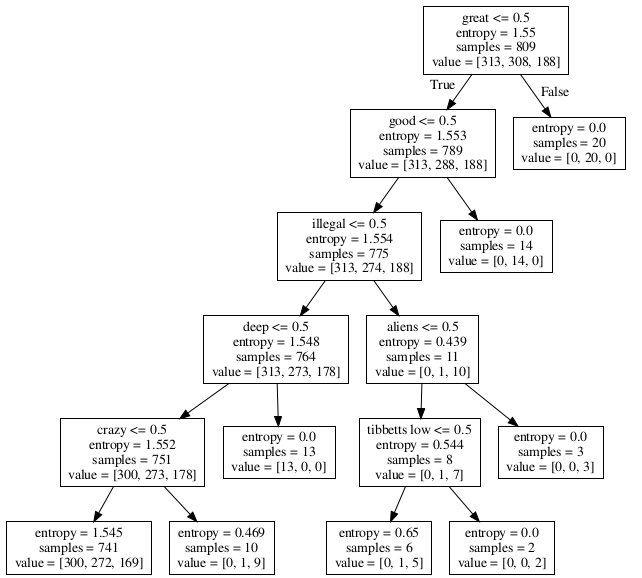
\includegraphics{imgs/1.png}
\caption{}
\end{figure}

\begin{itemize}
\tightlist
\item
  fold = 2
\end{itemize}

\begin{figure}[H]
\centering
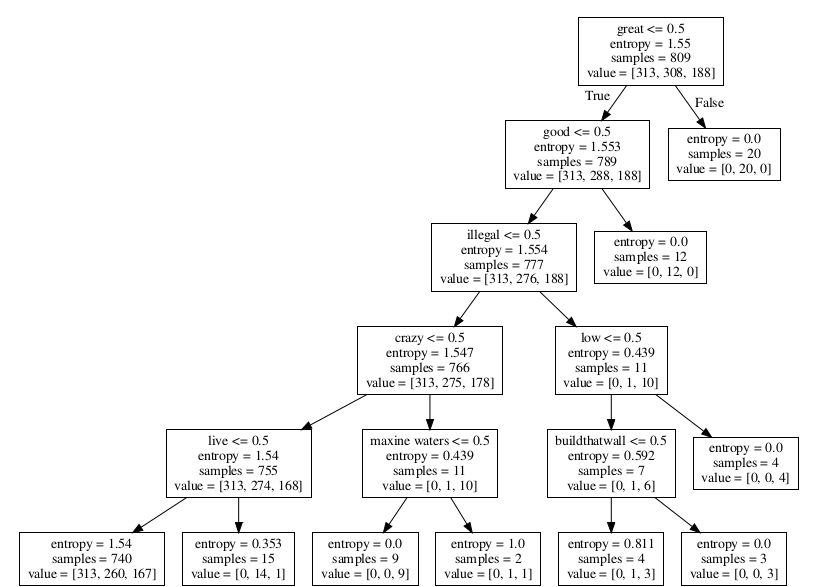
\includegraphics{imgs/2.png}
\caption{}
\end{figure}

\begin{itemize}
\tightlist
\item
  fold = 3
\end{itemize}

\begin{figure}[H]
\centering
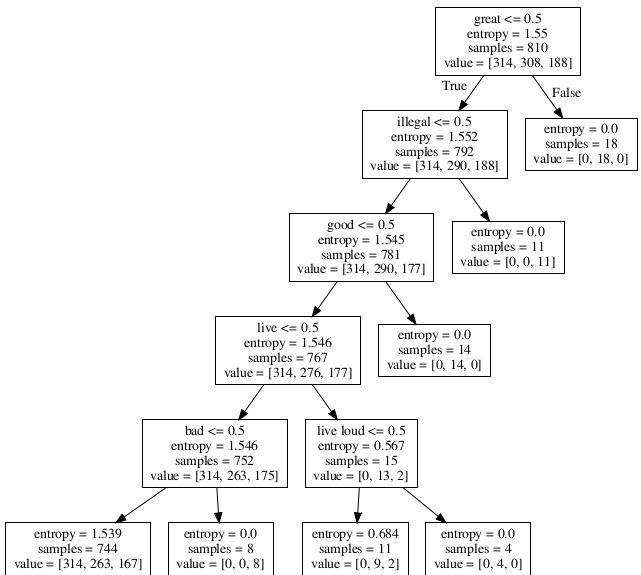
\includegraphics{imgs/3.png}
\caption{}
\end{figure}

\begin{itemize}
\tightlist
\item
  fold = 4
\end{itemize}

\begin{figure}[H]
\centering
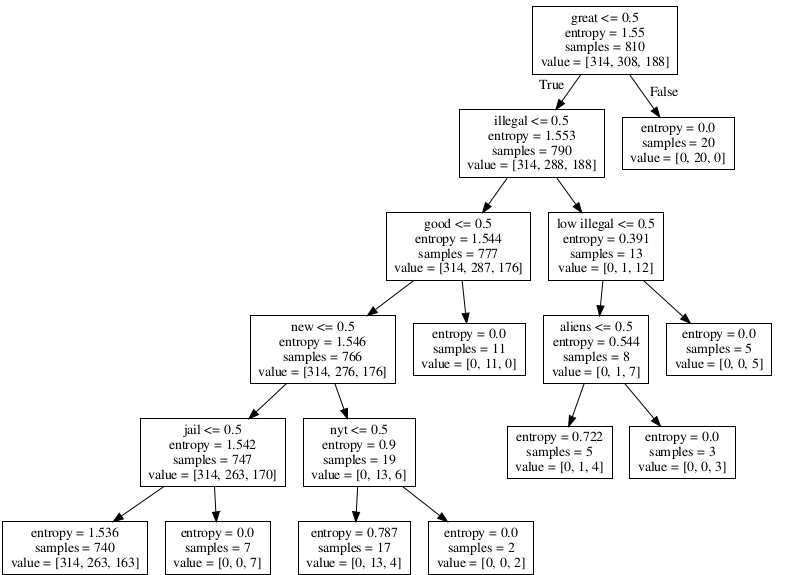
\includegraphics{imgs/4.png}
\caption{}
\end{figure}

\begin{itemize}
\tightlist
\item
  fold = 5
\end{itemize}

\begin{figure}[H]
\centering
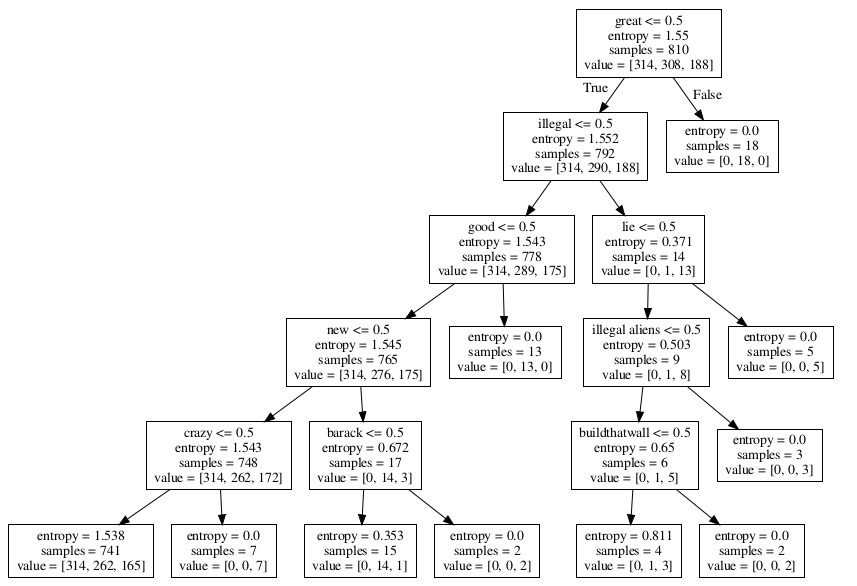
\includegraphics{imgs/5.png}
\caption{}
\end{figure}

    \begin{itemize}
\tightlist
\item
  Decision Trees of different folds share some similar features, for
  instance:

  \begin{itemize}
  \tightlist
  \item[*]
    \(great \le 5\) is the root node of all 5 trees
  \item[*]
    \(illegal \le 0.5, good \le 0.5\) also appears in all 5 trees
  \item[*]
    \(crazy \le 0.5, alien \le 0.5\) appears in not all 5 but also more
    than 1 tree
  \end{itemize}
\end{itemize}

    \subsubsection*{**Explore other possible
classifiers for the task}\label{explore-other-classifiers}

    \begin{Verbatim}[commandchars=\\\{\}]
{\color{incolor}In [{\color{incolor}68}]:} \PY{n}{vect} \PY{o}{=} \PY{n}{CountVectorizer}\PY{p}{(}
                  \PY{n}{analyzer}\PY{o}{=}\PY{l+s+s2}{\PYZdq{}}\PY{l+s+s2}{word}\PY{l+s+s2}{\PYZdq{}}\PY{p}{,} \PY{n}{ngram\PYZus{}range}\PY{o}{=}\PY{p}{(}\PY{p}{[}\PY{l+m+mi}{1}\PY{p}{,}\PY{l+m+mi}{2}\PY{p}{]}\PY{p}{)}\PY{p}{,} \PY{n}{tokenizer}\PY{o}{=}\PY{n}{nltk}\PY{o}{.}\PY{n}{word\PYZus{}tokenize}\PY{p}{,}
                 \PY{n}{preprocessor}\PY{o}{=}\PY{k+kc}{None}\PY{p}{,} \PY{n}{stop\PYZus{}words}\PY{o}{=}\PY{l+s+s1}{\PYZsq{}}\PY{l+s+s1}{english}\PY{l+s+s1}{\PYZsq{}}\PY{p}{,} \PY{n}{max\PYZus{}features}\PY{o}{=}\PY{l+m+mi}{3000}\PY{p}{)}
         \PY{n}{X\PYZus{}vect} \PY{o}{=} \PY{n}{vect}\PY{o}{.}\PY{n}{fit\PYZus{}transform}\PY{p}{(}\PY{n}{tagged}\PY{o}{.}\PY{n}{text}\PY{p}{)}\PY{o}{.}\PY{n}{todense}\PY{p}{(}\PY{p}{)}
         \PY{n}{y} \PY{o}{=} \PY{n}{tagged}\PY{o}{.}\PY{n}{sentiment}
\end{Verbatim}

    \begin{Verbatim}[commandchars=\\\{\}]
{\color{incolor}In [{\color{incolor}69}]:} \PY{k}{def} \PY{n+nf}{compare\PYZus{}classifiers}\PY{p}{(}\PY{n}{models}\PY{p}{,} \PY{n}{X}\PY{p}{,} \PY{n}{y}\PY{p}{)}\PY{p}{:}
             \PY{n}{CV} \PY{o}{=} \PY{l+m+mi}{5}
             \PY{n}{cv\PYZus{}df} \PY{o}{=} \PY{n}{pd}\PY{o}{.}\PY{n}{DataFrame}\PY{p}{(}\PY{n}{index}\PY{o}{=}\PY{n+nb}{range}\PY{p}{(}\PY{n}{CV} \PY{o}{*} \PY{n+nb}{len}\PY{p}{(}\PY{n}{models}\PY{p}{)}\PY{p}{)}\PY{p}{)}
             \PY{n}{entries} \PY{o}{=} \PY{p}{[}\PY{p}{]}
             \PY{k}{for} \PY{n}{model} \PY{o+ow}{in} \PY{n}{models}\PY{p}{:}
                 \PY{n}{model\PYZus{}name} \PY{o}{=} \PY{n}{model}\PY{o}{.}\PY{n+nv+vm}{\PYZus{}\PYZus{}class\PYZus{}\PYZus{}}\PY{o}{.}\PY{n+nv+vm}{\PYZus{}\PYZus{}name\PYZus{}\PYZus{}}
                 \PY{n}{accuracies} \PY{o}{=} \PY{n}{cross\PYZus{}val\PYZus{}score}\PY{p}{(}\PY{n}{model}\PY{p}{,} \PY{n}{X}\PY{p}{,} \PY{n}{y}\PY{p}{,} \PY{n}{scoring}\PY{o}{=}\PY{l+s+s1}{\PYZsq{}}\PY{l+s+s1}{accuracy}\PY{l+s+s1}{\PYZsq{}}\PY{p}{,} \PY{n}{cv}\PY{o}{=}\PY{n}{CV}\PY{p}{)}
                 \PY{k}{for} \PY{n}{fold\PYZus{}idx}\PY{p}{,} \PY{n}{accuracy} \PY{o+ow}{in} \PY{n+nb}{enumerate}\PY{p}{(}\PY{n}{accuracies}\PY{p}{)}\PY{p}{:}
                     \PY{n}{entries}\PY{o}{.}\PY{n}{append}\PY{p}{(}\PY{p}{(}\PY{n}{model\PYZus{}name}\PY{p}{,} \PY{n}{fold\PYZus{}idx}\PY{p}{,} \PY{n}{accuracy}\PY{p}{)}\PY{p}{)}
             \PY{n}{cv\PYZus{}df} \PY{o}{=} \PY{n}{pd}\PY{o}{.}\PY{n}{DataFrame}\PY{p}{(}\PY{n}{entries}\PY{p}{,} \PY{n}{columns}\PY{o}{=}\PY{p}{[}\PY{l+s+s1}{\PYZsq{}}\PY{l+s+s1}{model\PYZus{}name}\PY{l+s+s1}{\PYZsq{}}\PY{p}{,} \PY{l+s+s1}{\PYZsq{}}\PY{l+s+s1}{fold\PYZus{}idx}\PY{l+s+s1}{\PYZsq{}}\PY{p}{,} \PY{l+s+s1}{\PYZsq{}}\PY{l+s+s1}{accuracy}\PY{l+s+s1}{\PYZsq{}}\PY{p}{]}\PY{p}{)}
             \PY{n}{plt}\PY{o}{.}\PY{n}{figure}\PY{p}{(}\PY{n}{figsize}\PY{o}{=}\PY{p}{(}\PY{l+m+mi}{8}\PY{p}{,}\PY{l+m+mi}{8}\PY{p}{)}\PY{p}{)}
             \PY{n}{sns}\PY{o}{.}\PY{n}{boxplot}\PY{p}{(}\PY{n}{x}\PY{o}{=}\PY{l+s+s1}{\PYZsq{}}\PY{l+s+s1}{model\PYZus{}name}\PY{l+s+s1}{\PYZsq{}}\PY{p}{,} \PY{n}{y}\PY{o}{=}\PY{l+s+s1}{\PYZsq{}}\PY{l+s+s1}{accuracy}\PY{l+s+s1}{\PYZsq{}}\PY{p}{,} \PY{n}{data}\PY{o}{=}\PY{n}{cv\PYZus{}df}\PY{p}{)}
             \PY{n}{sns}\PY{o}{.}\PY{n}{stripplot}\PY{p}{(}\PY{n}{x}\PY{o}{=}\PY{l+s+s1}{\PYZsq{}}\PY{l+s+s1}{model\PYZus{}name}\PY{l+s+s1}{\PYZsq{}}\PY{p}{,} \PY{n}{y}\PY{o}{=}\PY{l+s+s1}{\PYZsq{}}\PY{l+s+s1}{accuracy}\PY{l+s+s1}{\PYZsq{}}\PY{p}{,} \PY{n}{data}\PY{o}{=}\PY{n}{cv\PYZus{}df}\PY{p}{,} 
                       \PY{n}{size}\PY{o}{=}\PY{l+m+mi}{8}\PY{p}{,} \PY{n}{jitter}\PY{o}{=}\PY{k+kc}{True}\PY{p}{,} \PY{n}{edgecolor}\PY{o}{=}\PY{l+s+s2}{\PYZdq{}}\PY{l+s+s2}{gray}\PY{l+s+s2}{\PYZdq{}}\PY{p}{,} \PY{n}{linewidth}\PY{o}{=}\PY{l+m+mi}{2}\PY{p}{)}
             \PY{n}{plt}\PY{o}{.}\PY{n}{xticks}\PY{p}{(}\PY{n}{rotation}\PY{o}{=}\PY{l+m+mi}{90}\PY{p}{)}
             \PY{n}{plt}\PY{o}{.}\PY{n}{show}\PY{p}{(}\PY{p}{)}
             
\end{Verbatim}

    \begin{Verbatim}[commandchars=\\\{\}]
{\color{incolor}In [{\color{incolor}97}]:} \PY{n}{models} \PY{o}{=} \PY{p}{[}
             \PY{n}{DecisionTreeClassifier}\PY{p}{(}\PY{n}{criterion} \PY{o}{=} \PY{l+s+s1}{\PYZsq{}}\PY{l+s+s1}{entropy}\PY{l+s+s1}{\PYZsq{}}\PY{p}{,}
                                             \PY{n}{random\PYZus{}state} \PY{o}{=} \PY{l+m+mi}{100}\PY{p}{,}
                                             \PY{n}{max\PYZus{}depth} \PY{o}{=} \PY{l+m+mi}{15}\PY{p}{,}
                                             \PY{n}{min\PYZus{}samples\PYZus{}leaf} \PY{o}{=} \PY{l+m+mi}{2}\PY{p}{)}\PY{p}{,}
             \PY{n}{RandomForestClassifier}\PY{p}{(}\PY{n}{random\PYZus{}state}\PY{o}{=}\PY{l+m+mi}{100}\PY{p}{,}
                                          \PY{n}{n\PYZus{}estimators}\PY{o}{=}\PY{l+m+mi}{50}\PY{p}{,} 
                                          \PY{n}{criterion}\PY{o}{=}\PY{l+s+s1}{\PYZsq{}}\PY{l+s+s1}{entropy}\PY{l+s+s1}{\PYZsq{}}\PY{p}{,} 
                                          \PY{n}{n\PYZus{}jobs}\PY{o}{=}\PY{l+m+mi}{4}\PY{p}{)}\PY{p}{,}
             \PY{n}{XGBoostClassifier}\PY{p}{(}\PY{n}{max\PYZus{}depth}\PY{o}{=}\PY{l+m+mi}{8}\PY{p}{,} \PY{n}{n\PYZus{}estimators}\PY{o}{=}\PY{l+m+mi}{5}\PY{p}{)}\PY{p}{,}
             \PY{n}{MultinomialNB}\PY{p}{(}\PY{p}{)}\PY{p}{,}
             \PY{n}{LogisticRegression}\PY{p}{(}\PY{n}{random\PYZus{}state}\PY{o}{=}\PY{l+m+mi}{0}\PY{p}{)}\PY{p}{,}
             \PY{n}{GradientBoostingClassifier}\PY{p}{(}\PY{p}{)}\PY{p}{,}
             \PY{n}{AdaBoostClassifier}\PY{p}{(}\PY{n}{n\PYZus{}estimators}\PY{o}{=}\PY{l+m+mi}{100}\PY{p}{,} \PY{n}{learning\PYZus{}rate}\PY{o}{=}\PY{l+m+mf}{0.1}\PY{p}{)}\PY{p}{,}
         \PY{p}{]}
         \PY{n}{compare\PYZus{}classifiers}\PY{p}{(}\PY{n}{models}\PY{p}{,} \PY{n}{X\PYZus{}vect}\PY{p}{,} \PY{n}{y}\PY{p}{)}
\end{Verbatim}

   

    \begin{center}
    \adjustimage{max size={0.8\linewidth}{0.8\paperheight}}{output_26_1.png}
    \end{center}
    { \hspace*{\fill} \\}
    
 

    % Add a bibliography block to the postdoc
    
    
    
    \end{document}
